\documentclass[12pt]{article}
\usepackage[left=12mm, top=0.5in, bottom=0.5in]{geometry}
\usepackage{amsmath}
\usepackage{mathtools}
\usepackage{amssymb}
\usepackage{pifont}
\usepackage{tikz-qtree}
\usepackage{tikz}
\usepackage{cite}
\usetikzlibrary{trees}

\geometry{left=15mm,right=15mm}

\newcommand{\cmark}{\ding{51}}%
\newcommand{\xmark}{\ding{55}}%
\newcommand\tab[1][1cm]{\hspace*{#1}}

\usepackage{hyperref}
\hypersetup{
    colorlinks=true,
    linkcolor=blue,
    filecolor=magenta,      
    urlcolor=cyan,
}
 
\urlstyle{same}

\begin{document}

\title{CS 440: Face and Digit Classification}
\author{Austin Bennett}
\maketitle


\section*{Observations}
\textbf{Note:} All data for the three tested classifiers (Naive Bayes, Perceptron, and K-Nearest Neighbor) are located below. \\
Also, \href{https://www.youtube.com/watch?v=YVwT--QiZGA}{Naive Bayes} and \href{https://www.youtube.com/watch?v=R2XgpDQro9k}{Perceptron}  were implemented exactly as described in the videos made by Professor Boularias.\\ \\
\textbf{Naive Bayes} \\
\tab One of the advantages of the Naive Bayes classifier that I observed while collecting data was that the computational time does not increase proportional to the number of data points tested. In the data provided, the difference in computation time was a mere 30\% increase from using 10\% of the data points to using 100\% of the data points. Without even having to understand the algorithm we can deduce that most, or at least a lot of the total computation required to fit the Naive Bayes classifier occurs regardless of the number of data points that are being trained on. This is great news if we have a massive data set but limited computational power, for example; a student in college using his own computer to apply machine learning algorithms to data sets. \\
\tab \textbf{Aside:} It is also worth noting that while there is a massive burst of test accuracy in the first 2500 data points, there is still a strong upward trend afterwards.
\begin{figure}[!htb]
	\centering
	\includegraphics[width=0.5\textwidth]{unreasonable_effectiveness_of_data.png}
	\caption{Learning Curves for Confusion Set Disambiguation}
\end{figure} \\
From Figure 1~\cite{Banko} we can see that given a large enough data set, many simplistic algorithms can actually approach extremely high test accuracy. Naive Bayes can in this case be implemented with basic features so as to generalize well to new data since it has had a massive amount of training data to practice on. All the while maintaining its originally low computation time and even less so due to the lack of necessity for complicated features.  \\
\tab Following this knowledge we can better understand why the Naive Bayes classifier performed "medicorely". In this project extremely simple features were implemented as to maintain a reasonable computation time and allow for appropriate testing of algorithms. With such a small data set, much more complicated features are required to have any deployable-level of accuracy.\\ \\
\textbf{Perceptron} \\
\tab Some interesting results arose from looking at the Perceptron data. For one, as opposed to the Naive Bayes classifier, the amount of computational time required is directly proportional to the number of data points used for the test. Another important fact to note is that while the training data was randomly sampled, the training data was not randomly sampled with stratification. In a multi-class data set like digits, this could be a very impactful alteration to improve test accuracy consistency (which my Perceptron data did not have). In the digits data set (as well as any data set) it is possible for there to be an uneven distribution of labels among all the possible classes, which can lead to a specific class being oversaturated in comparison to other classes in any given random sampling. \\
\tab As noted in the data section for Perceptron, the faces data was recorded using a maximum iteration of 4 for the perceptron algorithm. I decided on using 4 iterations after testing many different versions of the algorithm using various numbers of iterations ... all the way up to 1000 iterations. On average however, there was a very marginal increase in accuracy given these huge jumps in the number of iterations processed by the perceptron. As such I valued the extremely fast computation speed that also completed the required accuracy of $\geq$ 70\% over a marginally higher accuracy but also costing $\approx$ 300x more computation time. \\ \\
\textbf{K-Nearest Neighbor} \\
\tab The K-Nearest Neighbor classifier algorithm is extremely simple in that there is no actual training step to the algorithm, there is a simple distance calculation between the test data and our total known/labeled data. This simple distance calculation renders the algorithm quite prone to bad features and/or features that have little to no relevance. Compared to the strategy used for my perceptron and naive bayes classifiers, a much difference approach had to be taken. The extremely basic, but oversaturated method of detailing every single pixel as a feature according to whether it was a blank pixel or not was extremely detrimental in K-Nearest Neighbors algorithm. A much more relaxed set of features performed much better, such as breaking down the image into a 7x7 grid and counting the number of pixels in each grid.\\
\tab In addition to discovering the sensitivity of bad features in the algorithm, the sensitivity of the k value in the algorithm was unraveled. This sensitivty of the k value I presume is largely dependent on the fact that there were an uneven distribution of labels in the data sets used for this project. Precautions were taken to ensure that random samples of the training data were used, however these samples were not stratified. This lead to some inconsistency in the data, as it was quite possible for certain labels to have an unusually high percentage of the total labels in the training data. For example if a random sample was taken and 40\% of the labels were 9s and only 10\% of the labels were 7s, a major issue could arise whenever trying to classify a 7. Due to the nature of these two labels being very similar feature wise, a high k value in the algorithm would probably only classify 7s as 9s. This is not because the algorithm would think that the features of a 9 more closely represent that of the features of a 7, but simply because there was an oversaturation of 9s in the training data.	\\













\newpage
\section*{Naive Bayes Classifier - Digit}
python.exe .\textbackslash dataClassifier.py -c nb --data=digits -t 5000 -s 1000 \\
\begin{figure}[!htb]
	\centering
	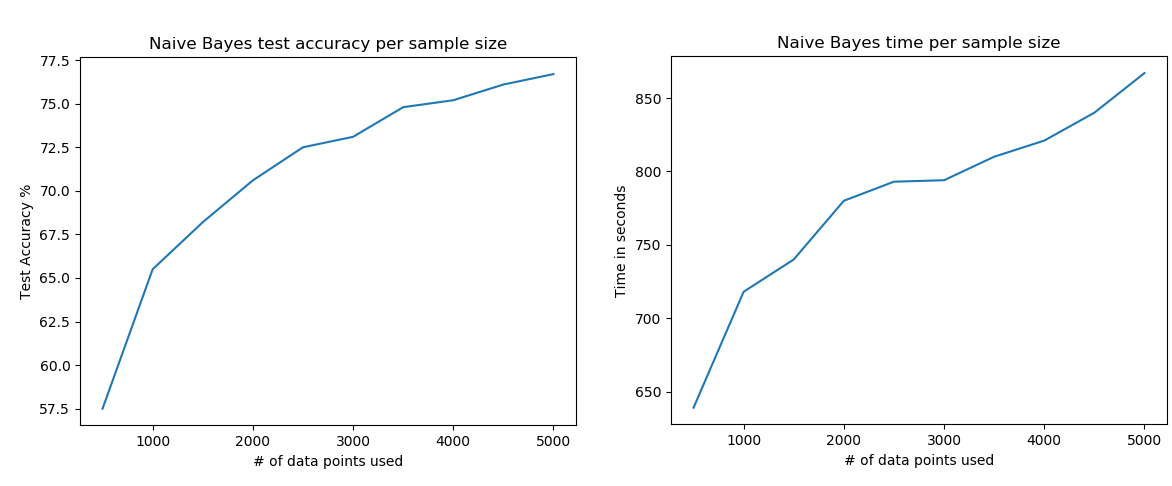
\includegraphics[width=1\textwidth]{nb_d.png}
\end{figure}
\section*{Naive Bayes Classifier - Face}
python.exe .\textbackslash dataClassifier.py -c nb --data=faces -t 451 -s 150 \\
\begin{figure}[!htb]
	\centering
	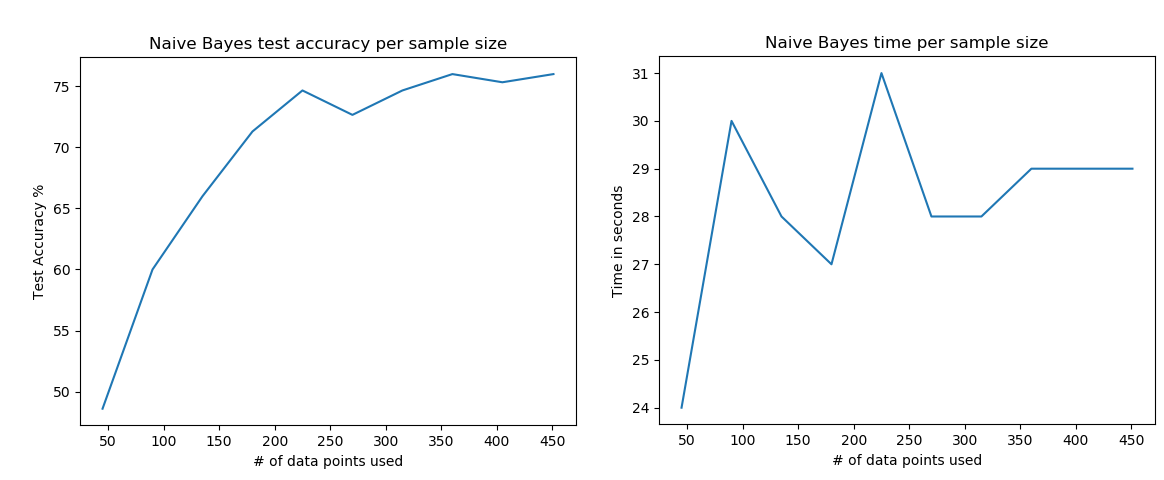
\includegraphics[width=1\textwidth]{nb_f.png}
\end{figure}
\newpage
\section*{Perceptron - Digit}
python.exe .\textbackslash dataClassifier.py -c perceptron --data=digits -t 5000 -s 1000 -i 10 \\
\begin{figure}[!htb]
	\centering
	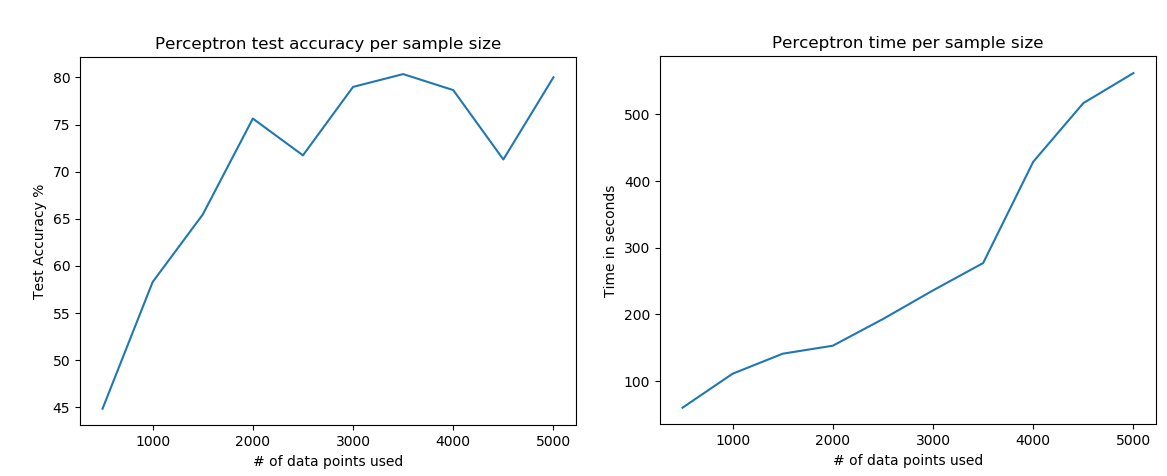
\includegraphics[width=1\textwidth]{perc_d.png}
\end{figure}
\section*{Perceptron - Face}
python.exe .\textbackslash dataClassifier.py -c perceptron --data=faces -t 451 -s 150 -i 4 \\
\begin{figure}[!htb]
	\centering
	\includegraphics[width=1\textwidth]{perc_f.png}
\end{figure}
\newpage
\section*{K-Nearest Neighbor Classifier - Digit}
python.exe .\textbackslash dataClassifier.py -c nearest --data=digits -t 5000 -s 1000 \\
\begin{figure}[!htb]
	\centering
	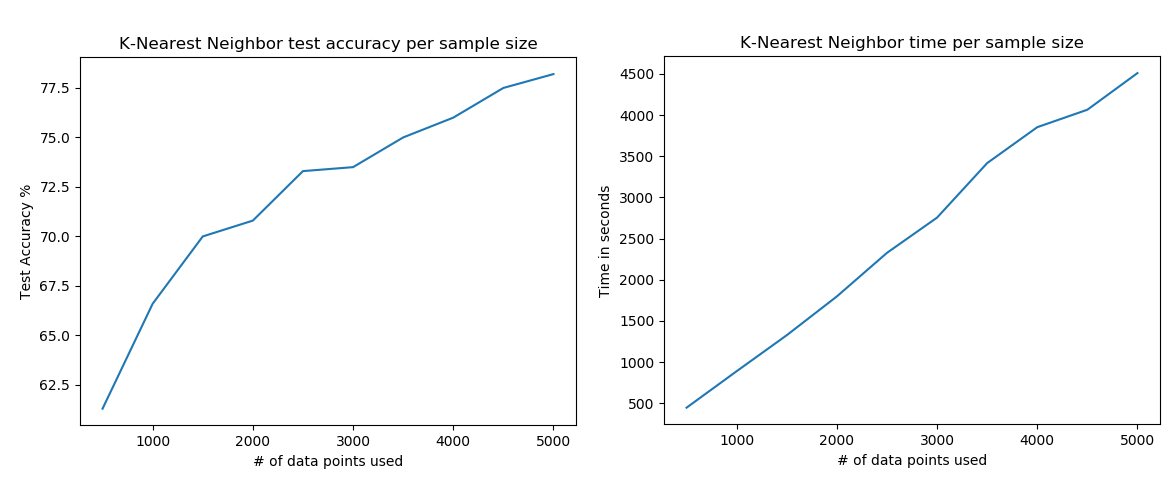
\includegraphics[width=1\textwidth]{knn_d.png}
\end{figure}
\section*{K-Nearest Neighbor Classifier - Face}
python.exe .\textbackslash dataClassifier.py -c nearest --data=faces -t 451 -s 150 \\
\begin{figure}[!htb]
	\centering
	\includegraphics[width=1\textwidth]{knn_f.png}
\end{figure}
\newpage
\bibliographystyle{plain}
\bibliography{mybib}








\end{document}